\documentclass[11pt]{article}
\usepackage[margin=0.9in]{geometry}
\usepackage{circuitikz}
\usepackage{tikz}
\usetikzlibrary{positioning}
\usepackage{array}
\usepackage{listings}
\usepackage{xcolor}

\lstset{basicstyle=\ttfamily\small, frame=single, backgroundcolor=\color{gray!8}}

\newcommand{\kmap}[5]{%
  % #1 title, #2-#5 four rows "a & b & c & d"
  \begin{tabular}{c}
  \textbf{#1}\\[2pt]
  \begin{tabular}{r|c c c c}
  \multicolumn{1}{r}{$A_2A_1\backslash B_2B_1$} & 00 & 01 & 11 & 10\\ \hline
  00 & #2\\
  01 & #3\\
  11 & #4\\
  10 & #5\\
  \end{tabular}
  \end{tabular}}

\begin{document}

\begin{center}
{\LARGE \texttt{final\_8} --- Gate-Level Redesign Workspace}\\[4pt]
{\large NAND / NOR / Inverter implementation of the 7-segment decoder}\\[2pt]
\textit{K-maps are pre-filled from your existing \texttt{top.v} truth table.
The minimization, groupings, and gate network are yours to derive.}
\end{center}

\section{Current design at a glance}

\begin{center}
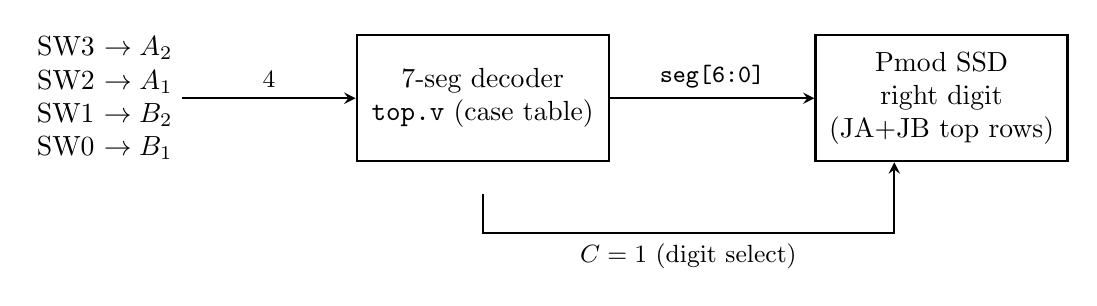
\begin{tikzpicture}[
  block/.style={draw, thick, minimum height=1.6cm, minimum width=3.2cm, align=center},
  >=stealth]
\node[block] (dec) {7-seg decoder\\ \texttt{top.v} (case table)};
\node[block, right=2.6cm of dec] (ssd) {Pmod SSD\\ right digit\\ (JA+JB top rows)};
\node[left=2.2cm of dec, align=right] (sw)
  {SW3 $\rightarrow A_2$\\ SW2 $\rightarrow A_1$\\ SW1 $\rightarrow B_2$\\ SW0 $\rightarrow B_1$};
\draw[->, thick] (sw) -- (dec) node[midway, above] {\small 4};
\draw[->, thick] (dec) -- (ssd) node[midway, above] {\small \texttt{seg[6:0]}};
\draw[->, thick] ([yshift=-0.4cm]dec.south) -- ++(0,-0.5) -| ([xshift=-0.6cm]ssd.south)
  node[pos=0.25, below] {\small $C = 1$ (digit select)};
\end{tikzpicture}
\end{center}

Signal-to-glyph mapping (bakes in the display's 180$^\circ$ mounting, per \texttt{arty.xdc}):
\texttt{seg[0]}\,=\,D (bottom), \texttt{seg[1]}\,=\,C (lower-right), \texttt{seg[2]}\,=\,E (lower-left),
\texttt{seg[3]}\,=\,G (middle), \texttt{seg[4]}\,=\,B (upper-right), \texttt{seg[5]}\,=\,F (upper-left),
\texttt{seg[6]}\,=\,A (top).

\section{K-maps (from your truth table --- circle your own groupings)}

Each map is one output bit of your \texttt{case} statement as a function of
$\{A_2, A_1, B_2, B_1\}$. Rows/columns are Gray-coded. Minimize each (SOP or POS),
then convert with DeMorgan (Section 3).

\begin{center}
\kmap{\texttt{seg[0]} --- viewed D (bottom)}
  {1 & 1 & 1 & 1}{1 & 0 & 1 & 1}{1 & 1 & 1 & 1}{1 & 1 & 1 & 0}
\hspace{1.2cm}
\kmap{\texttt{seg[1]} --- viewed C (lower-right)}
  {1 & 1 & 1 & 1}{1 & 1 & 1 & 0}{1 & 1 & 1 & 1}{1 & 0 & 1 & 1}

\vspace{0.9cm}
\kmap{\texttt{seg[2]} --- viewed E (lower-left)}
  {1 & 1 & 1 & 1}{1 & 0 & 0 & 1}{1 & 0 & 0 & 1}{1 & 1 & 1 & 0}
\hspace{1.2cm}
\kmap{\texttt{seg[3]} --- viewed G (middle)}
  {0 & 0 & 0 & 0}{0 & 0 & 1 & 1}{0 & 1 & 1 & 1}{0 & 1 & 1 & 1}

\vspace{0.9cm}
\kmap{\texttt{seg[4]} --- viewed B (upper-right)}
  {1 & 1 & 1 & 1}{1 & 1 & 1 & 1}{1 & 1 & 1 & 0}{1 & 1 & 0 & 1}
\hspace{1.2cm}
\kmap{\texttt{seg[5]} --- viewed F (upper-left)}
  {1 & 1 & 1 & 1}{1 & 0 & 0 & 0}{1 & 0 & 1 & 1}{1 & 0 & 1 & 1}

\vspace{0.9cm}
\kmap{\texttt{seg[6]} --- viewed A (top)}
  {1 & 1 & 1 & 1}{1 & 0 & 1 & 1}{1 & 1 & 1 & 1}{1 & 1 & 1 & 0}
\end{center}

\textit{Tip: several maps are mostly 1s --- consider grouping the 0s and building
the complement (POS $\rightarrow$ NOR-NOR), then compare gate counts against
SOP $\rightarrow$ NAND-NAND.}

\section{Gate symbols and DeMorgan conversion patterns}

\subsection*{Allowed gates}

\begin{center}
\begin{circuitikz}
\node[american nand port] (n1) at (0,0) {};
\node[below=2pt of n1] {NAND};
\node[american nor port] (n2) at (4,0) {};
\node[below=2pt of n2] {NOR};
\node[american not port] (n3) at (8,0) {};
\node[below=2pt of n3] {INV};
\end{circuitikz}
\end{center}

\subsection*{Textbook identities (generic --- not your solution)}

Two-level SOP maps to NAND-NAND; two-level POS maps to NOR-NOR:
\[
AB + CD \;=\; \overline{\overline{AB}\cdot\overline{CD}}
\qquad\qquad
(A{+}B)(C{+}D) \;=\; \overline{\overline{A{+}B} + \overline{C{+}D}}
\]

\begin{center}
\begin{circuitikz}
% NAND-NAND example: F = AB + CD
\node[american nand port] (g1) at (0,1.2) {};
\node[american nand port] (g2) at (0,-1.2) {};
\node[american nand port] (g3) at (2.6,0) {};
\draw (g1.out) -| ($(g3.in 1)+(-0.4,0)$) -- (g3.in 1);
\draw (g2.out) -| ($(g3.in 2)+(-0.4,0)$) -- (g3.in 2);
\draw (g1.in 1) -- ++(-0.4,0) node[left] {$A$};
\draw (g1.in 2) -- ++(-0.4,0) node[left] {$B$};
\draw (g2.in 1) -- ++(-0.4,0) node[left] {$C$};
\draw (g2.in 2) -- ++(-0.4,0) node[left] {$D$};
\draw (g3.out) -- ++(0.4,0) node[right] {$F = AB + CD$};
% NOR-NOR example: G = (A+B)(C+D)
\node[american nor port] (h1) at (8.5,1.2) {};
\node[american nor port] (h2) at (8.5,-1.2) {};
\node[american nor port] (h3) at (11.1,0) {};
\draw (h1.out) -| ($(h3.in 1)+(-0.4,0)$) -- (h3.in 1);
\draw (h2.out) -| ($(h3.in 2)+(-0.4,0)$) -- (h3.in 2);
\draw (h1.in 1) -- ++(-0.4,0) node[left] {$A$};
\draw (h1.in 2) -- ++(-0.4,0) node[left] {$B$};
\draw (h2.in 1) -- ++(-0.4,0) node[left] {$C$};
\draw (h2.in 2) -- ++(-0.4,0) node[left] {$D$};
\draw (h3.out) -- ++(0.4,0) node[right] {$G = (A{+}B)(C{+}D)$};
\end{circuitikz}
\end{center}

Complemented input literals come from inverters on $A_2, A_1, B_2, B_1$
(at most four inverters, shared across all seven outputs).

\subsection*{Structural Verilog primitives}

Output comes first; \texttt{nand}/\texttt{nor} take any number of inputs.

\begin{lstlisting}
wire nA2, nA1, nB2, nB1;
not  (nA2, A2);              // inverter
nand (w1, A2, nA1, B1);      // 3-input NAND
nand (seg0_x, w1, w2, w3);   // final NAND of a NAND-NAND pair
nor  (seg3_x, w4, w5);       // NOR
\end{lstlisting}

\vspace{0.5em}
\noindent\textit{When your gate-level \texttt{top.v} is written, run the testbench
first to prove equivalence with the case-statement version, then build and flash.}

\end{document}
